\setcounter{page}{1}
\fontsize{13}{15.6}\selectfont %font 13 Nhấn F6: Run -> F7: view
\begin{center}
	{\Large \bf \color{red} Bảng phân công công việc}
\end{center}
$$\begin{tabular}{|c|c|c|}
	\hline
	\textbf{STT}	&\textbf{Tên}	&\textbf{MSSV}	\\
	\hline
	1				& Nguyễn Văn A	&$2012001$	\\
	\hline
	2				& Nguyễn Văn B	&$2012002$	\\
	\hline
	3				& Nguyễn Văn C	&$2012003$	\\
	\hline
	4				& Nguyễn Văn D	&$2012004$	\\
	\hline
	5				& Nguyễn Văn C	&$2012005$	\\
	\hline
\end{tabular}$$
\begin{center}
	{\Large \bf \color{red} Nội dung câu hỏi}
\end{center}
\begin{enumerate}
	\item Đọc và trình bày lại các định lý ...
\end{enumerate}
\newpage
\tableofcontents %Mục lục
\newpage
\section{Câu 1}
\subsection{Câu a}
\noindent
Bài làm...\\[10pt]%Tùy khoảng cách mà cho số từ 6->10
Đây là hình ảnh
\begin{center}
	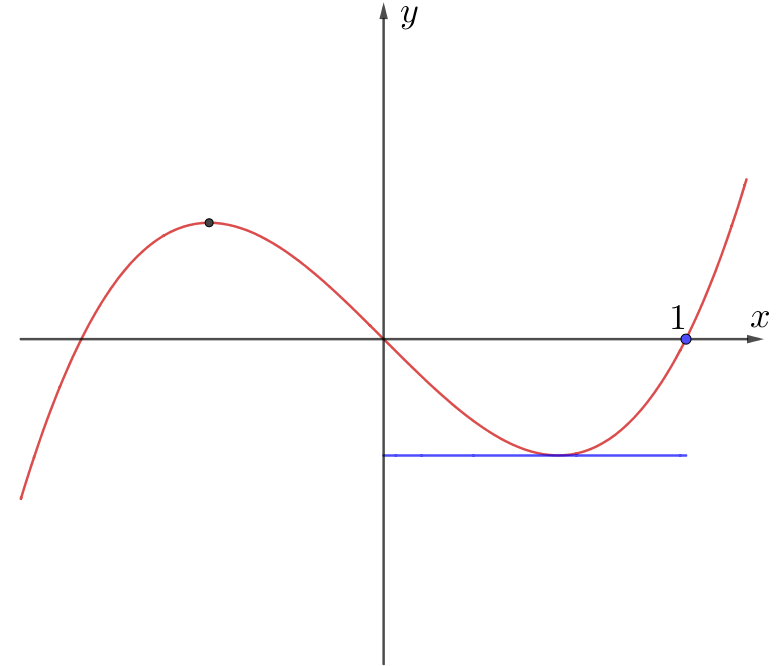
\includegraphics[scale=0.5]{pic/01}%F6
\end{center}
	Ví dụ thầy nhập vài                công thức cơ bản\\%Không ảnh hưởng bởi các dấu cách
$\int_0^1 x^2 dx = \dfrac{x^3}{3}+C$
$$\int_0^1 x^2 dx = \dfrac{x^3}{3}+C$$
$$\sum_{k=1}^{+\infty} k = +\infty$$
Thầy gửi thêm bảng công thức để dò nếu không biết kí hiệu đó.\\
Đây là một số công thức thông dụng: $\alpha$, $\beta$, $\lambda$. $\alpha$ Khi viết công thức phải cho trong dấu $x$\\
$$\boxed{\mbox{{\color{red}\bf Chúc các bạn hoàn thành bài tốt.}}}$$
\subsection{Câu b}
Bài làm...
\subsection{Câu c}
Bài làm...
\newpage
\section{Câu 2}
Bài làm...
\newpage
\section{Câu 3}
Bài làm...
\newpage
\section*{Tổng kết}
\addcontentsline{toc}{section}{\quad\  \bf Tổng kết}
Kết luận bài, bảng phân công nhiệm vụ.